\documentclass{patmorin}
\usepackage{pat,graphicx,amsopn}

\newcommand{\VG}{\mathit{VG}}
\newcommand{\EVG}{\mathit{EVG}}
\newcommand{\VSP}{\mathit{VSP}}
\newcommand{\Oe}{O_\epsilon}
\DeclareMathOperator{\start}{start}


\title{\MakeUppercase{Covering Visibility Polygons with Triangles:\newline
       Algorithms and Applications}}
\author{Joachim Gudmundsson\thanks{\affil{NICTA},
\email{joachim.gudmundsson@nicta.com.au}}\, 
       and Pat Morin\thanks{\affil{Carleton University},
\email{morin@scs.carleton.ca}}}

\begin{document}
\maketitle
\begin{abstract}
Let $S$ be a set of $n$ disjoint line segments in $\R^2$ and let $s$ be an
element of $S$.  An example due to O'Rourke (1987) shows that the subset,
$V_S(s)$, of $\R^2$ that is weakly visible from $s$ can have complexity
$\Omega(n^4)$.  In the current paper we show that $V_S(s)$ can always be
covered by a set $C_S(s)$ of $O(n^2)$ triangles.  More generally, we show
that the expected number of triangles needed to cover $V(S,s)$ for a random
element $s\in S$ is $O(n)$.

Storing the triangles of $C_S(s)$ in a partition tree (Welzl XX, Matou\v{s}ek
YY) yields an efficient data structure for testing if a query point is
contained in $V_S(s)$. Using random sampling, this yields an efficient
data structure for (additively) approximating the number of elements of
$S$ that are at least partially visible from a query point.  Furthermore,
%the structure of the triangles used in these coverings is such that
storing the $O(m)$ triangles of $\bigcup_{s\in S} C_S(s)$ in a partition
tree yields an efficient data structure for finding a 2-approximation
of the number of segments of $S$ partially visible from a query point.
This structure also yields an efficient output-sensitive data structure
for computing the visibility polygon of a point.  Here $m\le 2n^2-n$
is the number of edges in the visibility graph of $S$.
\end{abstract}

\section{Introduction}

Let $S$ be a set of $n$ closed line segments that are disjoint in the sense
that there are no two elements $s_1,s_2\in S$, with $s_1\neq s_2$, such
that the interior of $s_1$ and the interior of $s_2$ have a point in
common. 

Assume, without loss generality, that no segment in $S$ is vertical, so
that a point is \emph{above} a segment $s\in S$ if the point is above the
line that contains $s$.  Assume, furthermore, that $S$ contains 4 segments
that define a rectangle that contains all the elements of $S$ in its
interior.  

Two points $p,q\in\R^2$ are \emph{visible} (with respect to $S$) if the
open line segment $pq$ does not intersect any element of $S$.  A segment
$s\in S$ is \emph{visible} (with respect to $S$) from a point $p$ if there
exists a point $q\in s$ such that $p$ and $q$ are visible.

For a point $p\in\R^2$, the \emph{visibility region} or \emph{visibility
polygon} of $p$ (with respect to $S$) is defined as
\[
   V_S(p)=\{q\in\R^2:\mbox{$p$ and $q$ are visible (w.r.t. $S$)}\} 
      \enspace .
\]
For a segment $s\in S$, the \emph{visibility region} of $s$ (with respect
to $S$)
\[
   V_S(s)=\bigcup_{p\in s} V_S(p) \enspace 
\]
is the set of points in $\R^2$ that are visible from some point on $s$.
For a point $p$, $V_S(p)$ is connected and has complexity $O(n)$.  However,
for a segment $s$, $V_S(s)$ may be disconnected and can have $\Omega(n^4)$
components \cite{mXX,fXX}.

The \emph{visibility graph} $\VG(S)$ is a graph whose vertices are the $2n$
endpoints of the elements in $S$ and in which the edge $pq$ exists if and
only if the open line segment with endpoints $p$ and $q$ does not intersect
any (closed) segment in $S$ (see \figref{vg}.a).  It is well-known that the
number of edges in $\VG(S)$ is in $\Omega(n)\cap O(n^2)$.  Ghosh and Mount
\cite{gmXX} given an optimal $O(n\log n+ m)$ time algorithm to compute the
visibility graph of a set of $n$ line segments.  Here, and throughout the
remainder of the paper, $m$ is the number of edges of $\VG(S)$.

\begin{figure}
  \begin{center}
    \begin{tabular}{cc}
    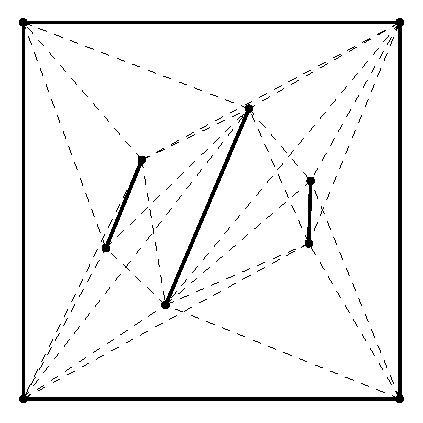
\includegraphics{vg} & 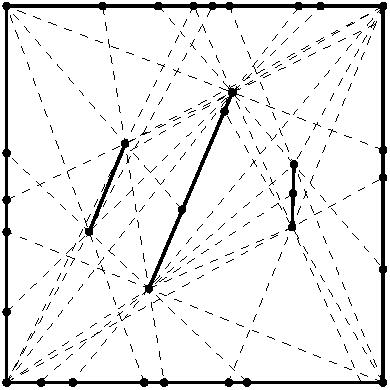
\includegraphics{evg} \\
    (a) & (b)
    \end{tabular}
  \end{center}
  \caption{The visibility graph and the extended visibility graph of a set
       of 7 line segments. (Segments are bold, graph edges are dashed.)}
  \figlabel{vg}
\end{figure}

Define the \emph{extended visibility graph} $\EVG(S)$ by adding $2m$ edges
and at most $2m$ vertices to $\VG(S)$ as follows (see \figref{vg}.b): For
each (directed) edge $uv$ in $\VG(S)$, extend a segment
$e_{uv}$ from $v$ in the direction $\overrightarrow{uv}$ until it
intersecting an element of $S$ at some point $w$.  If not already present,
then add the vertex $w$ to $\EVG(S)$ and add the edge $vw$ to $\EVG(S)$.

The union of the edges of $\EVG(S)$ and the segments in $S$ form a
1-dimensional set whose removal disconnects $\R^2$ into a set of
2-dimensional regions.  This set of 2-d regions is known as the
\emph{visibility space partition}, $\VSP(S)$ of $S$.  The regions of
$\VSP(S)$ are important because any region $R\in\VSP(S)$ does not intersect
the boundary of $V_S(s)$ for any element $s\in S$. That is, for any $p,q\in
R$ the set of segments of $S$ visible from $p$ is equal to the set of
segments of $S$ visible from $q$.  The region of $\VSP(S)$ that contains
$p$ determines all the combinatorial information about $V_S(p)$.

Note that $\VSP(S)$ is defined by $O(n^2)$ line segments, lines, and rays
so that it has complexity $O(n^4)$.  The example in \figref{quartic} shows
an example where this quartic complexity is achieved.

\begin{figure}
  \begin{center}
    
\includegraphics{quartic}
  \end{center}
  \caption{An example of a set $S$ where $\VSP(S)$ has complexity
$\Omega(n^4)$.  The $O(n)$ segments in the center define $\Omega(n^2)$
visibility graph edges whose extensions intersect in $\Omega(n^4)$ points.}
  \figlabel{quartic}
\end{figure}

\subsection{Previous Work}

There is a plethora of work on visibility in the plane.  This section
surveys only the work most relevant to the current paper.

The visibility space partition is bounded by a subset of the $O(n^2)$ lines
induced by pairs of endpoints in $S$. The arrangement of these lines
can be computed in $O(n^4)$ time using standard algorithms, and $\VSP(S)$
can be extracted in a further $O(n^4)$ time.  The example of O'Rourke shows
that this is optimal in the worst-case, since $\VSP(S)$ can have complexity
$\Omega(n^4)$. 

More generally, $\VSP(S)$ has complexity $O(m^2)$ where $m$ is the number
of edges in $\VG(S)$.  Ghosh and Mount \cite{gmXX} give an $O(n\log n + m)$
time algorithm to compute $\VG(S)$. Using this algorithm, one can compute
$\VSP(S)$ in $O(n\log n + m^2)$ time.

Motivated by applications in computer graphics, Fischer \etal\ \cite{fXX}
consider algorithms for exact and approximate \emph{visibility counting}:
Given a set of segments $S$, design a data structure that, given a query
point $p$, determines the number of segments of $S$ that are visible from
$p$.  Using $\VSP(S)$ and data structures for point location immediately
yields an $O(n^4)$ space $O(\log n)$ query time data structure for this
problem.  

Fischer \etal\ present several approximation data structures for visibility
counting.  One structure uses a cutting \cite{X} of $\VSP(S)$ to obtain a
data structure of size $O((m/r)^2)$ that answers queries in $O(\log n)$
time and approximates the visibility count up to an absolute error of $r$.
Another structure uses random sampling to obtain a data structure of size
$(m^2\log^{O(1)} n)/\ell$, has query time $\ell\log^{O(1)} n$ and approximates
the visibility count up to an absolute error of $\epsilon n$ for any
constant $\epsilon > 0$.

Pocchiola and Vegter \cite{pvXX} give an $O(m)$ space data structure that
can compute the visibility polygon from a query point $p$ in $O(k \log n)$
time.  Zarei and Ghodsi give an $O(n^3)$ space data structure that can
compute the visibility polygon in $O(k \log n)$ time.  More precisely, if
the segments of $S$ define a polygon with $h$ holes, the query time of
their structure is $O(\min\{h,k\}\log n + k)$, which improves the query
time of Pocchiola and Vegter when $h \ll k$.

If the segments of $S$ define a simple polygon then Bose \etal\ \cite{X}
and Guibas and Raghavan \cite{X} show that the complexity of $\VSP(S)$ is
only $O(n^3)$.  Using this fact, they give an $O(n^3)$ space data structure
that can compute the visibility polygon from a query point in $O(k + \log
n)$ time.  Aronov \etal \cite{axxX} give a data structure that reduces the
space to $O(n^2)$ at the cost of increasing the query time to $O(\log^2 n +
k)$.

\subsection{New Results}

The main result in the current paper is a proof that, for any $s\in S$,
there exists a set $C_S(s)$ of $O(m_s)$ triangles whose union is $V_S(s)$,
where $m_s$ is the number of edges of $\EVG(S)$ incident on $s$.  This
covering has an additional property that if we take the $O(m)$ size set
$C(S)=\bigcup_{s\in S}C_S(s)$ of triangles, then the number of triangles
containing any point $p\in\R^2$ is a 2-approximation to the number of
segments of $s$ that are visible from $p$.

These triangle-covering results have several applications that are obtained
by storing the triangles of $C_S(s)$ in a partition tree.   Here, and
throughout the remainder of the paper, $\epsilon > 0$ is a constant that
can be made arbitrarily small. To reduce clutter, we use the notation
$\Oe(f(n))=O(f(n)n^{\epsilon})$.

\paragraph{Visibility testing:} 
By storing the elements of $C_S(s)$ in a partition tree, we obtain an
$O(m_s^{1+\alpha})$ space data structure for testing if a query point $p$
is contained in $V_S(s)$ whose query time is $\Oe(m_s^{1/2(1-\alpha)})$.
Barring a major breakthrough on Hopcroft's Problem \cite{hXX,eXX},
this result is likely only a factor of $n^\epsilon$ from optimal.

For comparison purposes, the best known structure for this problem, as used
within the results of Fischer \etal\ \cite{fXX}, has size $O(m_{s}^2/\ell)$
and answers queries in $O(\ell\log n)$ time, where $\ell \ge 1$ is a
space/time tradeoff parameter of the data structure.  Taking
$\ell=\sqrt{n}$ yields a space of $O(m_s^{3/2})$ and a query time of
$O(\sqrt{m_s}\log n)$.  On the other hand, taking $\alpha=0$ in our data
structure yields an $O(m_s)$ space data structure with query time
$\Oe(\sqrt{m_s})$.

\paragraph{Visibility Counting --- Additive Approximation:}
Using random sampling, we obtain a data structure of size $O(n\log n)$
that approximates the number of segments of $S$ visible from any query
point in time $\Oe(\sqrt{n})$ to within an additive error of $\epsilon
n$.

For comparison purposes, the cutting-based data structure of Fischer
\etal\ \cite{fXX}, with $r=\epsilon n$, uses space $O((m/n)^2)\in
\Omega(n)\cap O(n^2)$ and has a query time of $O(\log n)$.  Using
the random sampling-based data structure of Fischer \etal\ with
$\ell=\sqrt{n}$ one obtains a data structure of size $(m^2\log^{O(1)}
n)/\sqrt{n}\in \Omega(n^{3/2})\cap O(n^{7/2}\log^{O(1)} n)$ with query
time $\sqrt{n}\log^{O(1)} n$.

\paragraph{Visibility Counting --- Relative Approximation:} 

Using space $O(m^{(1+\alpha)})\in O(n^{2(1+\alpha)})$ we obtain a data
structure that can $2$-approximate the number of segments of $S$ visible
from any query point in time $\Oe(m^{1/2(1-\alpha)})\in O(n^{1-\alpha})$.
This appears to be the first data structure of size $o(m^2)$ that can give
a relative approximation of the visibility count in $o(n)$ time.

%\paragraph{Visibility Polygon Queries:}
%With the same space (and same structure) used for 2-approximate visibility
%counting, we can compute the visibility polygon $V_S(p)$ of any query
%point $p$ in time $\Oe(n^{1-\alpha}) + O(k\log k)$ where $k$ is the
%size $V_S(p)$.

The remainder of the paper is organized as follows:  \Secref{covering}
proves results on covering visibility regions with triangles.
\Secref{applications} applies these results to obtain new results on
visibility testing and counting. \Secref{conclusions} summarizes and
concludes with open problems.

\section{Covering $V_S(s)$}
\seclabel{covering}

In this section we give an algorithm for covering the visibility region
$V_S(s)$ with triangles.  The number of triangles used in the covering is
bounded by $O(n+m_s)$ where $m_s$ is the number of edges of $\EVG(S)$ that
are incident to $s$.  We will show how to cover the portion
$V^+_S(s)\subseteq V_S(s)$ in the halfplane bounded from below by the
supporting line of $s$ with a set $C^+_S(s)$ of triangles.  The
complementary part $V^-_S(s)=V_S(s)\setminus V^+_S(s)$ can be covered with
a set $C^-_S(s)$ using symmetric algorithm.

The covering algorithm works by sweeping a point $p$ from left to right
across the segment $s$.  Events in this sweep occur at the vertices
$p_1,\ldots,p_{m'_s}$ of $\VSP(S)$ incident on $s$, in their left to right
order, so that $p_1$ and $p_{m'_s}$ are the left and right endpoints,
respectively, of $s$.

Let $e$ be an edge of $V^+_S(p)$ that is collinear with $p$ and such that the
interior of $V^+_S(p)$ is to the right of $e$. We call such an edge an
\emph{active edge} of $V^+_S(p)$.  Active edges are important because, as $p$
moves to the right, they uncover regions of $\R^2$ which may not have been
previously visible.  See \figref{alg}.a.

Let $q$ be the lower endpoint of $e$ and note that $q$ is an endpoint of
some segment $s\in S$. Consider what happens to $e$ as the viewpoint $p$
moves left to right along $s$, but does not cross any edge of $\EVG(S)$
collinear with $q$.  As $p$ moves left to right, the edge $e$ remains
collinear with $p$ and $q$ and sweeps over a triangle $\Delta_e$ whose
lowest vertex is $q$.  This continues until, at some point, the point $p$
reaches an edge of $\VSP(S)$ incident on $q$.   See \figref{alg}.b.

Algorithmically, the cover $C^+_S(s)$ is constructed as follows: Initially
$p=p_1$ is the left endpoint of $S$.  We compute the visibility polygon
$V^+_S(p)$, whose boundary is a sequence of $m_p=O(n)$ edges that alternate
between subsegments of the elements of $S$ and segments collinear with $p$
and an endpoint of an element of $S$.  This polygon can be covered in a
natural way with $m_p/2$ non-overlapping triangles, each of which has $p$
as a vertex (see \figref{alg}.a). These $m/2$ triangles are added to
$C^+_S(s)$.  After computing $V^+_S(p)$ we identify its active edges, and with
each active edge $e$ we store the value $\start(e)=p_1$.

\begin{figure}
  \begin{center}
    \begin{tabular}{ccc}
      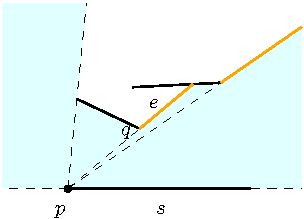
\includegraphics{alg-1} &
      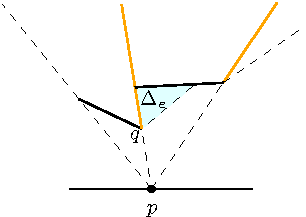
\includegraphics{alg-2} &
      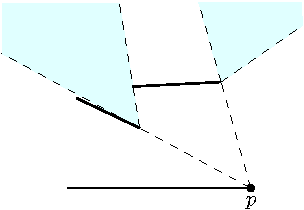
\includegraphics{alg-3} \\
      (a) & (b) & (c)
    \end{tabular}
  \end{center}
  \caption{The algorithm for covering $V^+_S(s)$ with triangles processing
           the events at (a)~$p_1$, (b)~$p_2$ and (c)~$p_3$.  
           Active edges are shown in orange and triangles in the covering
are shown at the time they are added to the covering.}
  \figlabel{alg}
\end{figure}

Next, we begin sweeping $p$ from left to right, pausing at the vertices
$p_2,\ldots,p_{m'_s}$ as we go.  Upon reaching a vertex $p_i$, we process
the edges of $\EVG(S)$ incident on $p_i$ one at a time.\footnote{For
segments in sufficiently general position, $p_i$, $1<i<m_s$ will be
incident to only one edge of $\EVG(S)$, but the covering algorithm does not
require this.}  Let $e'$ be an edge of $\EVG(S)$ incident on $p_i$. If $e'$
is collinear with an active edge $e$ of $V^+_S(p)$ then we generate a new
triangle $\Delta_e$ for $C^+_S(s)$.  The lowest vertex of $\Delta_e$ is the
lower endpoint $q$ of $e$. $\Delta_e$ is bounded by two lines
$\ell_1,\ell_2$, both of which contain $q$, and where $\ell_1$ contains
$p=p_i$ and $\ell_2$ contains $\start(e)$ .  The third side of $\Delta_e$
is bounded by the segment in $S$ incident on $e$ and furthest from $p$. See
\figref{alg}.b.

Finally, the visibility polygon $V^+_S(p)$ is updated in the neighbourhood of
$e$, which possibly creates a new active edge $f$ incident to $q$.  In this
case, $f$ is marked as active and $\start(f)=p_i$.  The exact nature of
this update depends on the relative locations of the two segments that
define $e'$.  The three possible cases are illustrated in \figref{cases}.

\begin{figure}
  \begin{center}
    \begin{tabular}{|c|c|c|}
      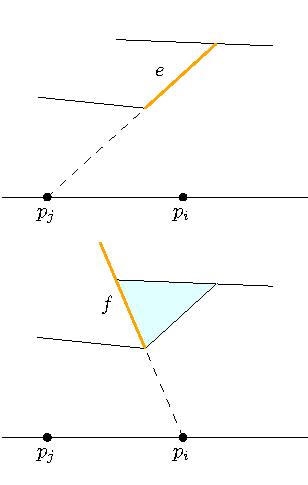
\includegraphics{case-a} &
      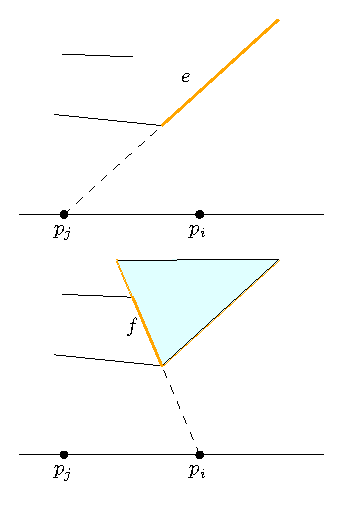
\includegraphics{case-b} &
      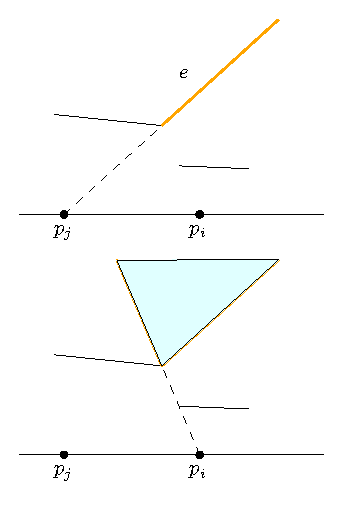
\includegraphics{case-c} \\
      (a) & (b) & (c)
    \end{tabular}
  \end{center}
  \caption{The three cases that occur when processing an edge of $\EVG(S)$
incident on $p_i$.  Here, $\start(e)=p_j$.}
  \figlabel{cases}
\end{figure}

Note that an important event, but which requires no special handling occurs
at the right endpoint of $s$ when $p=p_{m_s}$.  In this case, each active
edge of $V^+_S(p)$ generates a triangle that is added to the set $C^+_S(s)$.
See \figref{alg}.c.

We now prove the correctness of the above algorithm:

\begin{lem}\lemlabel{cover}
Let $C^+_S(s)$ be the set of triangles generated by running the above
algorithm.  Then $\cup C^+_S(s) = V^+_S(s)$ and $|C^+_S(s)|\le m_s$ where
$m_s$ is the number of edges of $\VSP(S)$ incident on $s$.
\end{lem}

\begin{proof}
To prove the bound on the size, first observe that the initial visibility
polygon $V^+_S(p_1)$ has size that is bounded by the degree of $p_1$ in
$\VSP(S)$.  Furthermore, at each event point $p_i$, $i>1$, the number of
triangles added to $C^+_S(s)$ is at most the number of edges of $\VSP(S)$
incident to $p_i$.  Therefore, the total number of triangles in $C^+_S(s)$
is at most the number of edges of $\VSP(S)$ incident to $s$.

The fact that $\cup C^+_S(s)\subseteq V^+_S(s)$ follows immediately
from the easily verifiable fact that each triangle added to $C^+_S(s)$
contains only points visible from some point on $p\in s$.

To prove that $C^+_S(s)$ covers $V^+_S(s)$, consider a point $r\in V^+_S(s)$.  If
$r$ is visible from $p_1$ then $r$ is contained in one of the triangles
added during the initialization of the algorithm.  Otherwise, there exists
some point $p'\in s$ with minimum $x$-coordinate such that $r$ is visible
from $p'$.  It follows that $p'$ and $r$ are collinear with a vertex $q$ of
some segment $s'\in S$ and that $q$ is on the segment $p'r$ (see
\figref{cover-proof}.a).  Then $q$ is an endpoint of an active edge $e$ of
$V^+_S(p')$ with $\start(e)$ to the left of $p'$.  Since every active edge
eventually adds a triangle to $C^+_S(s)$, there is some $p_i$ to the right of
$p'$ that adds a triangle $\Delta_e$ to $C^+_S(s)$ that contains $r$ (see
\figref{cover-proof}.b).  Since this is true for every point $r\in V^+_S(s)$,
we conclude that $\cup C^+_S(s)\supseteq V^+_S(s)$, and hence $\cup C^+_S(s)=
V^+_S(s)$.  
\end{proof}

\begin{figure}
  \begin{center}
    \begin{tabular}{cc}
      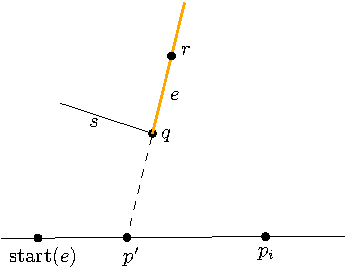
\includegraphics{cover-proof-a} &
      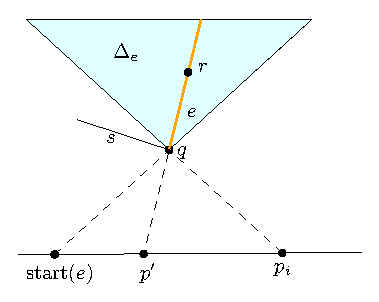
\includegraphics{cover-proof-b} \\
      (a) & (b)
    \end{tabular}
  \end{center}
  \caption{Proving that $C^+_S(s)$ covers $V^+_S(s)$.}
  \figlabel{cover-proof}
\end{figure}

Next we show that, in a global sense, the number of triangles containing a
point $p\in\R^2$ gives an approximation to the number of segments of $S$
that are visible from $p$. Let $C_S(s) = C^+_S(s)\cup C^-_S(s)$.

\begin{lem}\lemlabel{count}
Let $C(S)=\bigcup_{s\in S} C_S(s)$ and let $p$ be any point in $\R^2$ that
is not on the boundary of any triangle in $C(S)$.  If $m_p$ is the number
of segments in $S$ (partially) visible from $p$ and $m'_p$ is the number
of triangles in $C(S)$ that contain $p$, then $m_p \le m'_p \le 2m_p$.
\end{lem}

\begin{proof}
Let $C_p\subseteq C(S)$ be the set of triangles in $C(S)$ that contain
$p$, and let $S_p$ be the number of segments in $S$ that are (partially)
visible from $p$.  The lower bound on $m'_p$ is trivial:  For every
segment $s$ that is partially visible from $p$, $V_S(s)$ contains $p$,
so, by \lemref{cover}, $C_S(s)$ contributes at least one triangle to $C(S)$.

To prove the upper bound, we describe a mapping $f: C_p \rightarrow S_p$
that is \emph{$2$-to-one}; for every $s\in S_p$, there exists at most 2
triangles $\Delta\in C_p$ such that $f(\Delta)=s$. The existence of $f$
then proves the upper bound.

Let $\Delta\in C(S)$ be some triangle that contains $p$ and suppose that
$\Delta\in C_S(s)$ for some $s\in S$ that is, without loss of generality,
below $p$.  If $\Delta$ is incident on $s$ (\figref{counting}.a), then $\Delta$ was added to
$C_S(s)$ as part of $V_S(p)$ where $p$ was the left endpoint of $s$.  In
this case, we set $f(\Delta)=s$.  Otherwise, $\Delta$ was created when
sweeping $s$ with $p$ and some active edge $e$ of $V_S(p)$ generated
$\Delta$ (\figref{counting}.b).  The vertex $q$ of $\Delta$ that is closest to $s$ is incident on a
segment $s'\in S$.  In this case $f(\Delta)=s'$.

\begin{figure}
  \begin{center}
    \begin{tabular}{cc}
      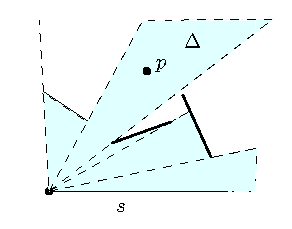
\includegraphics{counting-a} &
      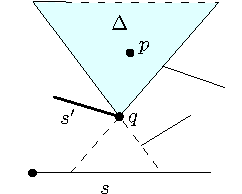
\includegraphics{counting-b} \\
      (a) $f(\Delta)=s$ & (b) $f(\Delta)=s'$
    \end{tabular}
  \end{center}
  \caption{The mapping $f$ takes $\Delta$ onto (a)~$s$ and (b)~$s'$.}
  \figlabel{counting}
\end{figure}

We now argue that $f$ is 2-to-one.  Let $s\in S$ be some segment and
suppose, without loss of generality, that $p$ is above $s$.  Consider a
triangle $\Delta \in f^{-1}(s)$ and observe that, by the definition of $f$,
$\Delta$ has a vertex that is an endpoint of $s$.

Note that there is at most one triangle in $C_S(s)$ that maps to $s$, and
this triangle exists precisely if $p$ is visible from the left endpoint of
$s$.  All that remains to show is that there is at most one additional
segment $s'\in S$, $s'\neq s$ such that $C_S(s')$ contains a triangle
$\Delta$ with $f(\Delta)=s$.

Let $\Delta$ be such a triangle and suppose that $\Delta$ is incident to
the endpoint $q$ of $s$.  Refer to \figref{count-right}.  The triangle
$\Delta$ was generated by an active edge when processing $s'$.  In
particular, there is a subsegment $p_j p_i\subseteq s'$ such that an active
edge $e$ of $V^+_S(p)$ sweeps over $\Delta$ when $p$ travels from $p_j$ to
$p_i$. (Note, $p_j=\start(e)$.) this implies that $p_i$ and $p_j$ are below
$s$. Since $p$ travels from left to right along $e$, this implies that $q$
is the right endpoint of $s$ because, otherwise, $e$ would not be an active
edge of $V^+_S(p)$.

\begin{figure}
  \begin{center}
    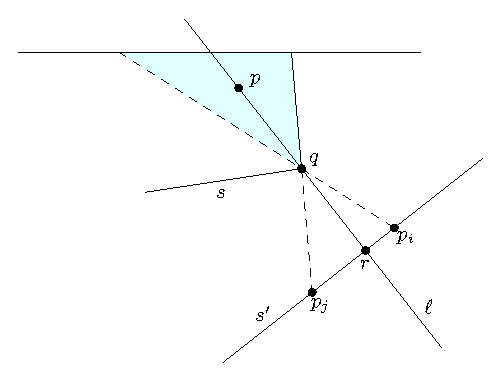
\includegraphics{count-right}
  \end{center}
  \caption{At most one triangle in $f^{-1}(s)$ is incident to the right
           endpoint of $S$.}
  \figlabel{count-right}
\end{figure}

Thus far, we have established that at most one triangle in $f^{-1}(s)$ is
incident to the left endpoint of $s$.  To see that at most one triangle
($\Delta$, discussed above) is incident to the right endpoint of $s$,
suppose by way of contradiction that there are two such triangles $\Delta$
and $\Delta'$ with $\Delta\in C_S(s')$ and $\Delta'\in C_S(s'')$.
Consider the line $\ell$ through $p$ and $q$.  Observe that $\ell$
intersects both $s$ and $s'$, in two points $r$ and $r'$, respectively. But
this is not possible since then one of $r$ or $r'$ does not see the
endpoint $q$.
\end{proof}

\paragraph{Remark:}
The condition, in \lemref{count}, that $p$ is not on the boundary of
any triangle in $C_S(s)$ is unnecessary if we take a little care.
In particular, the mapping $f$ maps triangles to the endpoints of
segments.  The set $C_S(v)$ of triangles mapped to a particular endpoint
$v$ all have $v$ as a vertex and no two triangles in $C_S(v)$ share an
interior point.  This means that we can define each triangle in $C_S(v)$
to either include or exclude some of its edges or vertices so that the
triangles are disjoint but their union remains unchanged. This yields
a set of (partially open) triangles $C'(S)$ for which \lemref{count}
holds for any point $p\in\R^2$

\section{Applications}
\seclabel{applications}

In this section, we consider applications of \lemref{cover} and
\lemref{counting} to some visibility counting problems considered by
Fischer \etal\ \cite{fXX}.  These applications rely on data structures for
triangle-inclusion counting.  The principle behind these data structures
are well-established, but we review them here for the sake of completeness.

Given a set $T$ of triangles, we say that a point $p\in\R^2$ \emph{crosses}
$T$ if there exists $\Delta_1,\Delta_2\in T$ such that $p\in\Delta_1$ and
$p\not\in\Delta_2$.

\begin{lem}\lemlabel{partition}[Matou\v{s}ek XXXX]
  Given a set $T$ of $\ell$ triangles, and an integer $r$, there exists
  a partition of $\mathcal{T}=\{T_1,\ldots,T_r\}$ of $T$ such that
  \begin{enumerate}
    \item for each $i\in\{1,\ldots,r\}$, $|T_i| \le 2\ell/r$, and
    \item for any point $p\in\R^2$, $p$ crosses at most $O(r^{1/2})$ 
          sets in $\mathcal{T}$.
  \end{enumerate}
  Furthermore, the partition $\mathcal{T}$ can be computed by a randomized
  algorithm in $\Oe(\ell)$ time.
\end{lem}

To use \lemref{partition}, we construct a partition tree in which every
node has at most  $r$ children and has depth at most $(c \log \ell)/(\log
(r/2))$.  This tree has at most $\Oe(\ell^c)$ leaves and Part~1 of the
lemma implies that each leaf stores at most $\Oe(\ell^{1-c})$ triangles.
The triangles within each leaf are stored in a quadratic size data
structure that can answer queries in $O(\log \ell)$ time.  This gives a
total storage of $\Oe(\ell^{2-c})$.  Part~2 of the lemma ensures that the
number of nodes visited when answering a query, and hence the total query
time, is $\Oe(\ell^{c/2})$.  Rewriting these values gives

\begin{thm}\thmlabel{partition-tree}
Given a set $T$ of $\ell$ triangles, there exists a data structure
of size $\Oe(\ell^{1+\alpha})$ that, for any query point $p\in\R^2$,
can determine the number of triangles of $T$ that contain $p$ in
$\Oe(\ell^{(1-\alpha)/2})$ time.
\end{thm}

\subsection{Visibility Testing}

Our first application follows immediately by storing the triangles of
\lemref{cover} in the partition tree of \thmref{partition-tree}.  This
yields our first result:

\begin{thm}\thmlabel{containment}
Given a set $S$ of $n$ disjoint line segments and a marked segment
$s\in S$, there exists a data structure of size $\Oe(m_s^{1+\alpha})$
that can test if any query point $p\in\R^2$ is contained in $V_S(s)$,
in $\Oe(m_s^{(1-\alpha)/2})$ time.
\end{thm}

Barring a breakthrough on Hopcroft's Problem, \thmref{containment} is
probably near-optimal.  Given a set $L$ of $n$ lines, it's possible to
construct a set of $3n+1$ segments $s_0,\ldots,s_{3n}$ such that a query
point $q$ sees $s_0$ if and only if $q$ lies on one of the lines in $L$.
Currently, partition trees are the most efficient method of solving this
problem.  A solution with $o(n^{4/3})$ preprocessing and $o(n^{1/3})$ query
time would give a $o(n^{4/3})$ solution to Hopcroft's Problem.

FIXME: Can we construct this data structure in output-sensitive time?

\subsection{Visibility Counting -- Absolute Approximation}



\subsection{Visibility Counting -- Relative Approximation}

\subsection{Visibility Polygon Queries}





\end{document}
